%----------------------------------------------------------------------------------------
%    PACKAGES AND THEMES
%----------------------------------------------------------------------------------------

\documentclass[aspectratio=169,xcolor=dvipsnames,10pt]{beamer}
\usetheme{SimplePlus}

\usepackage{hyperref}
\usepackage{graphicx} % Allows including images
\usepackage{booktabs} % Allows the use of \toprule, \midrule and \bottomrule in tables
\usepackage{bbm}
\usepackage{bm}
\usepackage{mathtools}
\usepackage{amsthm}
\usepackage{tikz-cd}

\theoremstyle{definition}
\newtheorem{proposition}{Proposition}

\usepackage[square,numbers]{natbib}
\newcommand*{\QEDA}{\hfill\ensuremath{\blacksquare}}%
\newcommand*{\QEDB}{\hfill\ensuremath{\square}}%

%----------------------------------------------------------------------------------------
%    TITLE PAGE
%----------------------------------------------------------------------------------------

\title{Data Visualization From a Category Theory Perspective}
\subtitle{}

\author{Davi Sales Barreira, Asla Medeiros e Sá}

\institute
{
    FGV - EMAp, IMPATech
}
\date{\today} % Date, can be changed to a custom date

%----------------------------------------------------------------------------------------
%    PRESENTATION SLIDES
%----------------------------------------------------------------------------------------
\setbeamertemplate{blocks}[default]
\setbeamercolor{block title}{fg=white, bg=RoyalBlue}
\setbeamercolor{block body}{fg=black, bg=white}

\begin{document}

\begin{frame}
    % Print the title page as the first slide
    \titlepage
\end{frame}

%------------------------------------------------
\section{Introduction to the Course}
\begin{frame}[fragile]{Motivation}
  Balance expressiveness and abstraction in data visualization
  frameworks.
	\vspace{3mm}
	\begin{figure}[H]
		\begin{center}
			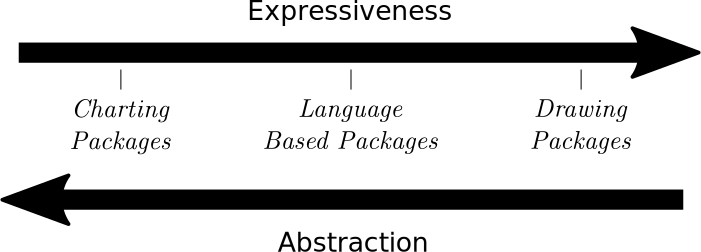
\includegraphics[width=0.8\textwidth]{./figures/expressiveness.pdf}
		\end{center}
        % \caption{Rotated histogram aligned with second main PCA axis.}
		\label{fig:rotated-histogram}
	\end{figure}
\end{frame}

\begin{frame}[fragile]{Motivation}
    How can we represent complex visualizations without resorting to low-level specifications?
	\vspace{3mm}
	\begin{figure}[H]
		\begin{center}
			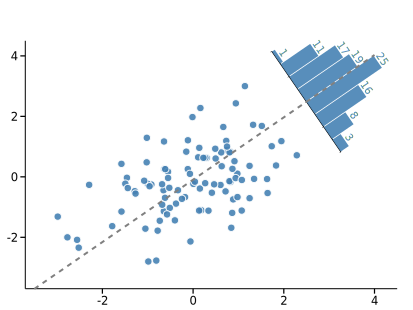
\includegraphics[width=0.45\textwidth]{./figs/pca.pdf}
		\end{center}
        \caption{Rotated histogram aligned with second main PCA axis.}
		\label{fig:rotated-histogram}
	\end{figure}
\end{frame}

\begin{frame}[fragile]{Motivation}
    How can we represent complex visualizations without resorting to low-level specifications?
	\vspace{3mm}
	\begin{figure}[H]
		\begin{center}
			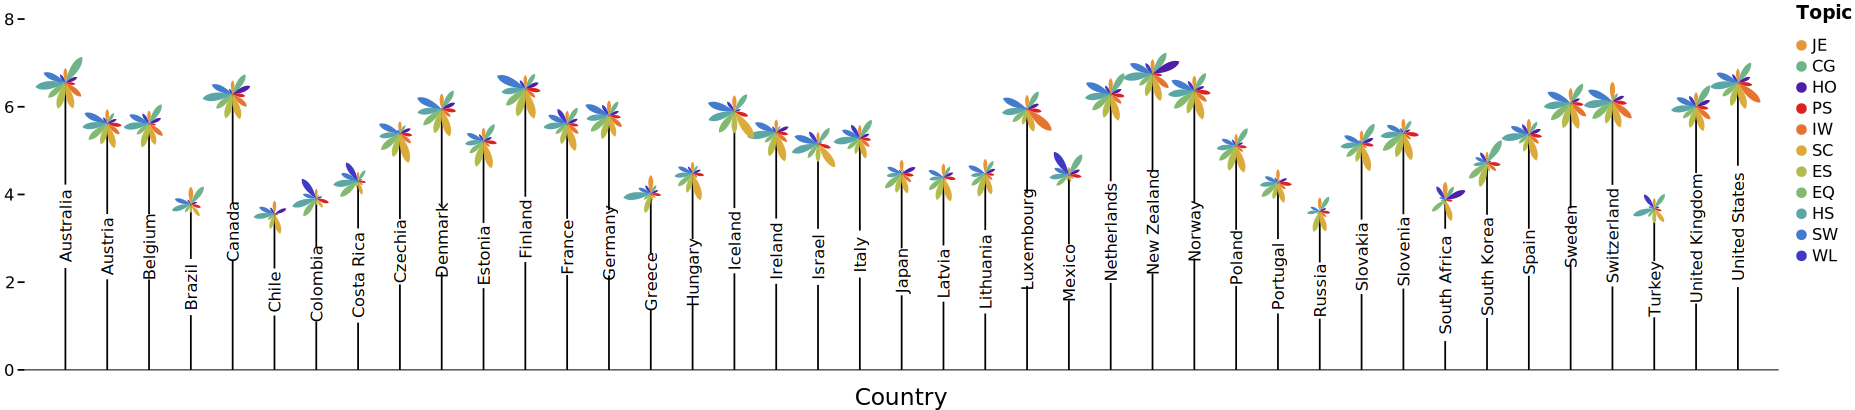
\includegraphics[width=1.\textwidth]{./figs/moritz.pdf}
		\end{center}
        \caption{OECD Better Life Index visualization \citet{oecd}.}
		\label{fig:rotated-histogram}
	\end{figure}
\end{frame}

\begin{frame}[fragile]{Overview}
    \begin{itemize}
        \item \textbf{Day 1}: Basics of Category Theory
        \item \textbf{Day 2}: Programming with Category Theory
        \item \textbf{Day 3}: Data Visualization Theory
        \item \textbf{Day 4}: Data Visualization + Categorical Programming
    \end{itemize}
\end{frame}
%------------------------------------------------

\begin{frame}{Table of contents}
	% \setbeamertemplate{section in toc}[sections numbered]
	% \setbeamertemplate{subsection in toc}[subsections numbered]
	% \setbeamerfont{subsection in toc}{size=\small}
	% \tableofcontents[sectionstyle=show, subsectionstyle=show]
    \begin{enumerate}
        \item What are Categories?
        \item Examples of Categories
        \item Universal Constructions
        \item Functors
        \item Natural Transformations
        \item Monoids and Monads
        \item F-Algebras and F-Coalgebras
    \end{enumerate}
\end{frame}

\section{Category Theory}
\begin{frame}[fragile]{Why Category Theory?}
	\textbf{Category Theory} is a branch of mathematics that
	studies general abstract structures through their relationships.
	\vspace{3mm}

	\textbf{Origin: }Samuel Eilenberg e Saunders Mac Lane - 1940
	\vspace{3mm}

	As pointed by \citet{fong2019invitation}, Category Theory is unmatched
	in its ability to organize and relate abstractions.

	\vspace{3mm}
	\begin{figure}[H]
		\begin{center}
			\includegraphics[width=0.40\textwidth]{./figures/category-triad.pdf}
		\end{center}
	\end{figure}
\end{frame}

\begin{frame}[fragile]{What are Categories?}
	Category Theory is a branch of mathematics that
	studies general abstract structures through their relationships.

	\begin{definition}[Category]
        \begin{itemize}
            \item A collection of objects $\mathrm{Ob}_{\mathcal{C}}$.
            \item A collection of morphisms $\mathrm{Hom}_{\mathcal{C}}$, where each morphism has a source object and a target object. $\mathrm{Hom}_{\mathcal{C}}(A, B)$ is the collection of morphisms going from object $A$ to object $B$.
            \item A binary operation $\circ : \mathrm{Hom}_{\mathcal{C}}(A, B) \times \mathrm{Hom}_{\mathcal{C}}(B, C) \to \mathrm{Hom}_{\mathcal{C}}(A, C)$ such that:
            \begin{enumerate}
                \item \textbf{Associative}: $(h \circ g) \circ f = h \circ (g \circ f)$.
                \item \textbf{Identity}: Every object has an identity morphism $1_A \in \mathrm{Hom}_{\mathcal{C}}(A, A)$.
            \end{enumerate}
        \end{itemize}
	\end{definition}
\end{frame}

\begin{frame}[fragile]{What are Categories?}

    \begin{definition}[Small and Locally Small Category]
        A category $\mathcal C$ is \textit{small} if $\text{Ob}_\mathcal C$ and
        $\text{Hom}_\mathcal C$ are sets. A category $\mathcal C$ is \textit{locally small} if
        for any $A, B \in \text{Ob}_\mathcal C$, then
        $\text{Hom}_\mathcal C(A,B)$ is a set. Note that a small category is also locally small.
    \end{definition}

    Note that when talking about $\text{Ob}_\mathcal C$ and $\text{Hom}_\mathcal C$, we didn't say
    that they were sets, instead we called them \textit{classes}. The reason for
    this lies in the foundations of Set Theory. There are collections in mathematics
    that are ``larger'' than sets, e.g. the ``set'' of all sets, which itself cannot be a set,
    otherwise it would incur in a paradox (Russell's Paradox). A way to deal
    with this is making a distinction between classes and sets.
    This point is quite technical; readers interested in understanding this nuance can check books such as \citet{borceux1994handbook}.
\end{frame}

\begin{frame}[fragile]{Examples of Categories}
    The category $\mathbf{1}$ consists of $\text{Ob}_{\mathbf{1}} := \{A\}$ and $\mathrm{Hom}_{\mathbf{1}} = \mathrm{id}_A$.

	\begin{figure}[H]
		\begin{center}
			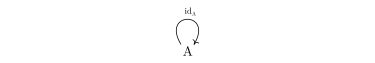
\includegraphics[width=1.0\textwidth]{./figs/1Cat.pdf}
		\end{center}
	\end{figure}

\end{frame}

\begin{frame}[fragile]{Examples of Categories}
	The category $\bm 2$ consists of $\text{Ob}_{\bm 2} := \{A, B\}$ and $\text{Hom}_{\bm 1} = \{id_A, id_B, f\}$,
	where $f:A \to B$.
	The diagram for such category is shown below.
	\begin{figure}[H]
		\begin{center}
			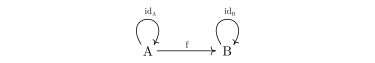
\includegraphics[width=1.00\textwidth]{./figs/2Cat.pdf}
		\end{center}
		\caption{Category $\bm 2$.}
		\label{fig:2Cat}
	\end{figure}
\end{frame}

\begin{frame}[fragile]{Examples of Categories}
	The category $\bm 3$ has three morphisms besides the identities. The morphisms are
	$f$, $g$ and their composition $g \circ f$. The figure below
	illustrates the category with all its morphisms.
	\bigskip
	\begin{figure}[H]
		\begin{center}
			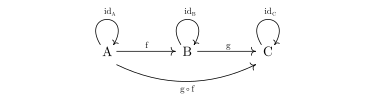
\includegraphics[width=1.00\textwidth]{./figs/3Cat.pdf}
		\end{center}
		\caption{Category $\bm 3$ showing all morphisms.}
		\label{fig:3Catcomplete}
	\end{figure}
\end{frame}

\begin{frame}[fragile]{Examples of Categories}
    When drawing categories, it is common to omit
    the identity and/or composition morphism. From here on,
    we do the same, whenever the context is clear.
	\bigskip
	\begin{figure}[H]
		\begin{center}
			\includegraphics[width=1.00\textwidth]{../notebooks/3Catsimple.pdf}
		\end{center}
		\caption{Category $\bm 3$ omitting morphisms.}
		\label{fig:3Catcomplete}
	\end{figure}
\end{frame}

\begin{frame}[fragile]{Examples of Categories}
	The discrete category $\mathbf{\underline{N}}$ is the category with $N$ objects
    and $\text{Hom}_{\mathbf{\underline{N}}} := \{id_1,...,id_N\}$. An example of this category is
	illustrated below.
	\bigskip
	\begin{figure}[H]
		\begin{center}
			\includegraphics[width=0.80\textwidth]{../notebooks/DiscreteCategory.pdf}
		\end{center}
        \caption{Category $\mathbf{\underline{N}}$.}
		\label{fig:3Catcomplete}
	\end{figure}
\end{frame}

\begin{frame}[fragile]{Examples of Categories}
        Given a category \(\mathcal{C}\) and an object \(S\) of this category, we can define a slice category \(\mathcal{C} / S\), where:
        \begin{itemize}
            \item The objects are tuples \((A, f)\) where \(A\) is an object in \(\mathcal{C}\) and \(f: A \to S\) is a morphism.
            \item A morphism \(\varphi_{(A, B)} : (A, f) \to (B, g)\) is equivalent to a morphism \(\varphi \in \text{Hom}_{\mathcal{C}}(A, B)\) such that \(f = g \circ \varphi\).
        \end{itemize}
	\begin{figure}[H]
		\begin{center}
			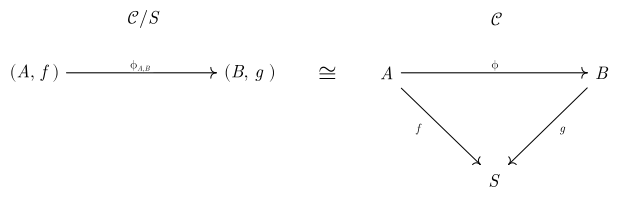
\includegraphics[width=0.70\textwidth]{./figs/SliceCategory.pdf}
		\end{center}
		\caption{Example of slice category.}
		\label{fig:slice}
	\end{figure}
\end{frame}

\begin{frame}[fragile]{Examples of Categories}
    \begin{definition}[Subcategory]
        Let $\mathcal C$ be a category. A \textit{subcategory} $\mathcal S$ of $\mathcal C$ is such that
        \begin{enumerate}[(i)]
            \item $\text{Ob}_\mathcal S \subseteq \text{Ob}_\mathcal C$;
            \item For every $A,B \in \text{Ob}_\mathcal S$, we have $\text{Hom}_\mathcal S(A,B) \subseteq \text{Ob}_\mathcal C(A,B)$;
            \item Composition and identity in $\mathcal S$ are the same as in $\mathcal C$, restricted to morphisms and objects of $\mathcal S$.
        \end{enumerate}

        A subcategory $\mathcal S$ is said to be \textit{wide} if $\text{Ob}_\mathcal S = \text{Ob}_\mathcal C$,
        and it is said to be \textit{full} if for every $A,B \in \text{Ob}_\mathcal S$, then 
        $\text{Hom}_\mathcal S(A,B) = \text{Hom}_\mathcal C(A,B)$.
        % Finally, a subcategory is \textit{thin} if
        % for every $A,B \in \text{Ob}_\mathcal S$ the set $\text{Hom}_\mathcal S(A,B)$ has only a single morphism.
    \end{definition}
\end{frame}

\begin{frame}[fragile]{Examples of Categories}
    \begin{definition}[Dual Category]
        Given a category $\mathcal C$, the dual (opposite) category $\mathcal C^{op}$ is defined as:
        \begin{itemize}
            \item $\text{Ob}_{\mathcal C^{op}} = \text{Op}_\mathcal C$;
            \item For every morphism $f:A\to B$ in $\mathcal C$, have an equivalent morphism $f^{op}:B \to A$ in $\mathcal C^{op}$;
            \item The composition in $\mathcal C^{op}$ satisfies $f^{op} \circ g^{op} = (g \circ f)^{op}$.
        \end{itemize}
    \end{definition}
	\begin{figure}[H]
		\begin{center}
			\includegraphics[width=0.35\textwidth]{../notebooks/DualCategory.pdf}
		\end{center}
		\caption{Example of dual category.}
		\label{fig:dual}
	\end{figure}
\end{frame}

\begin{frame}[fragile]{Examples of Categories}
	Here are some more interesting
	categories:
	\begin{enumerate}[1.]
		\item $\mathbf{Set}$ which is the category of sets, where the objects are sets and the morphisms are functions between sets.
		\item $\mathbf{Top}$ is the category where topological spaces are the objects and continuous functions are the morphisms.
		\item $\mathbf{Vec}_\mathbb F$ is the category where vector spaces over field $\mathbb F$ are the objects,
		      and linear transformations are the morphisms.
		\item $\mathbf{Mon}$ is the category of monoids, where morphisms are monoid homormophisms.
	\end{enumerate}
\end{frame}

\begin{frame}[fragile]{Isomorphisms, monomorphism and epimorphism}
    A very important definition in Category Theory is the notion of isomorphism. In Set Theory,
    we say that two sets are isomorphic if there is a bijective function between them. Yet, this
    concept is not restricted to Set Theory and can be generalized in Category Theory as follows:
	\begin{definition}[Categorical Isomorphism]
        Let $\mathcal C$ be a category with $X,Y \in Ob_\mathcal C$ and $f \in \text{Hom}_\mathcal C (X,Y)$.
        \begin{enumerate}[(i)]
            \item We say that $f$ is \textit{left invertible} if there exists $f_l \in \text{Hom}_\mathcal C (Y,X)$ such
                  that $f_l \circ f = id_X$;
              \item We say that $f$ is \textit{right invertible} if there exists $f_r \in \text{Hom}_\mathcal C (Y,X)$ such
                  that $f \circ f_r = id_Y$;
            \item We say that $f$ is invertible if it's both left and right invertible.
        \end{enumerate}
	\end{definition}
    \textbf{Exercise}: Prove that in the category $\mathbf{Set}$, the categorical isomorphism is equivalent to
    the set theoretic isomorphism.
\end{frame}

% \begin{frame}[fragile]{Isomorphisms, monomorphism and epimorphism}
%     A very important definition in Category Theory is the notion of isomorphism. In Set Theory,
%     we say that two sets are isomorphic if there is a bijective function between them. Yet, this
%     concept is not restricted to Set Theory and can be generalized in Category Theory as follows:
% 	\begin{definition}[Categorical Isomorphism]
%         Let $\mathcal C$ be a category with $X,Y \in Ob_\mathcal C$ and $f \in \text{Hom}_\mathcal C (X,Y)$.
%         \begin{enumerate}[(i)]
%             \item We say that $f$ is \textit{left invertible} if there exists $f_l \in \text{Hom}_\mathcal C (Y,X)$ such
%                   that $f_l \circ f = id_X$;
%               \item We say that $f$ is \textit{right invertible} if there exists $f_r \in \text{Hom}_\mathcal C (Y,X)$ such
%                   that $f \circ f_r = id_Y$;
%             \item We say that $f$ is invertible if it's both left and right invertible.
%         \end{enumerate}
% 	\end{definition}
%     \begin{proof}
%         Let $f: A \to B$ be a morphism in $\mathbf{Set}$. We will show that $f$ is a categorical isomorphism if and only if it is a bijection.

%         \textbf{(⟹) If $f$ is a categorical isomorphism, then $f$ is a bijection.}  

%         Since $f$ is an isomorphism, there exists a morphism $g: B \to A$ such that:
%         \[
%         g \circ f = \text{id}_A, \quad f \circ g = \text{id}_B.
%         \]

%         - \textit{$f$ is injective}: Suppose $f(x) = f(y)$. Applying $g$ to both sides, we get  
%           \[
%           g(f(x)) = g(f(y)).
%           \]  
%           Since $g \circ f = \text{id}_A$, this simplifies to  
%           \[
%           x = y.
%           \]  
%           Thus, $f$ is injective.  

%         - \textit{$f$ is surjective}: For every $b \in B$, we have  
%           \[
%           f(g(b)) = \text{id}_B(b) = b.
%           \]  
%           This shows that every element of $B$ has a preimage in $A$, proving that $f$ is surjective.  

%         Since $f$ is both injective and surjective, it is a bijection.

%         \textbf{(⟸) If $f$ is a bijection, then it is a categorical isomorphism.}  

%         Since $f$ is a bijection, it has an inverse function $f^{-1}: B \to A$ such that  
%         \[
%         f^{-1} \circ f = \text{id}_A, \quad f \circ f^{-1} = \text{id}_B.
%         \]  
%         This precisely means that $f$ is an isomorphism in the categorical sense.

%         Thus, we have shown that a categorical isomorphism in $\mathbf{Set}$ is the same as a bijection. $\square$
%     \end{proof}
% \end{frame}
% \begin{frame}[fragile]{Isomorphisms, monomorphism and epimorphism}
%     A partially ordered set (poset) is defined by a tuple $(P, \leq)$, where $P$ is a set of values and
%     $\leq$ is a binary relation satisfying reflexivity, antisymmetry and transitivity.
%     \begin{enumerate}[(i)]
%         \item For $a,b \in P$, if $a\leq b$ and $b \leq c$, then $a \leq c$;
%         \item For every $a \in P$, $a \leq a$.
%     \end{enumerate}

%     The \textbf{Poset} category has partially ordered sets as objects and monotone maps as morphisms,
%     i.e., maps $f : X \to Y$, such that for each $x, x' \in X$ with $x \leq x'$ in $X$, we have $f(x) \leq f(x')$ in $Y$.

% \end{frame}

\begin{frame}[fragile]{Isomorphisms, monomorphism and epimorphism}
	\begin{definition}[Monomorphism]
        In a given category $\mathcal C$, a morphism $m:X\to Y$ is said to be a monomorphism (monic),
        if for every $A \in \text{Ob}_\mathcal C$ and $f,g:A \to X$ we have that:
        $$
        m\circ f = m\circ g \implies f = g.
        $$
	\end{definition}
	\begin{definition}[Epimorphism]
        In a given category $\mathcal C$, a morphism $e:X\to Y$ is said to be an epimorphism (epic),
        if for every $A \in \text{Ob}_\mathcal C$ and $f,g:A \to X$ we have that:
        $$
        f \circ e = g \circ e \implies f = g.
        $$
	\end{definition}
\end{frame}

\begin{frame}[fragile]{Isomorphisms, monomorphism and epimorphism}
    \begin{proposition}
        The following properties on monomorphism and epimorphism are true:
        \begin{enumerate}[1.]
            \item $f$ left-invertible $\implies$ $f$ is monic. The converse is not true.
            \item $f$ right-invertible $\implies$ $f$ is epic. The converse is not true.
            \item $f$ invertible $\implies$ $f$ is monic and epic. The converse is not true.
            \item $f$ monic and right-invertible $\implies $ $f$ is isomorphism.
            \item $f$ epic and left-invertible $\implies $ $f$ is isomorphism.
        \end{enumerate}
    \end{proposition}
    \begin{proof}
        Left as exercise.
    \end{proof}
\end{frame}

% \begin{frame}[fragile]{Isomorphisms, monomorphism and epimorphism}
%     \begin{proposition}
%         The following properties on monomorphism and epimorphism are true:
%         \begin{enumerate}[1.]
%             \item $f$ left-invertible $\implies$ $f$ is monic. The converse is not true.
%             \item $f$ right-invertible $\implies$ $f$ is epic. The converse is not true.
%             \item $f$ invertible $\implies$ $f$ is monic and epic. The converse is not true.
%             \item $f$ monic and right-invertible $\implies $ $f$ is isomorphism.
%             \item $f$ epic and left-invertible $\implies $ $f$ is isomorphism.
%         \end{enumerate}
%     \end{proposition}
%     \begin{proof}
%         1. Note $f:A \to B$ left-invertible implies that there exists a $f_l:B \to A$ such that
%         $f_l \circ f = id$. Hence, for a $g:B\to C$ and $h: B \to C$, if
%         \begin{displaymath}
%             f \circ g = f \circ h,
%         \end{displaymath}
%         then we have that
%         \begin{displaymath}
%             f_l \circ f \circ g = f_l \circ f \circ h \implies g =h.
%         \end{displaymath}
%         To show that the converse is false, consider the category $\mathbf{2}$ (Figure \ref{fig:2Cat}). Note that
%         $f:A\to B$ is monic, since the only morphism that composes with $f$ is
%         $id_A$ and $id_B$. Yet, note that $f$ is not left invertible, since there isn't even
%         a morphism from $B$ to $A$.

%         2. Use the same argument, but reversing the order of the compositions.
%         For the converse, again consider the same category $\mathbf{2}$. Note that
%         $f:A\to B$ is epic, but it's not right invertible.

%         3. True since invertible means left and right invertible.

%         4. Since $f:A \to B$ right invertible, then there exists $f_r:B \to A$
%         such that $f \circ f_r = id_B$. Thus,
%         \begin{displaymath}
%             id_B \circ f = (f \circ f_r) \circ f =
%             f \circ (f_r \circ f) =
%             f \circ id_A \implies f_r \circ f = id_A.
%         \end{displaymath}
%         5. Same argument.
%     \end{proof}
% \end{frame}

\begin{frame}[fragile]{Universal Constructions}
	Objects defined in terms of existence and
	uniqueness of morphisms are known as \textbf{universal constructions}.
	\begin{definition}[Zero, Initial and Terminal]
		Let $\mathcal C$ be a category.
		\begin{enumerate}[1.]
			\item An object $I \in \text{Ob}_\mathcal C$ is \textit{initial} if for every $A \in \text{Ob}_\mathcal C$,
			      there is exactly one morphism from $I$ to $A$. Thus, from $I$ to $I$ there is only the identity.
			\item An object $T \in \text{Ob}_\mathcal C$ is \textit{terminal} if for every $A \in \text{Ob}_\mathcal C$,
			      there is exactly one morphism from $A$ to $T$. Thus, from $I$ to $I$ there is only the identity.
			\item An object is \textit{zero} if it is both terminal and initial.
		\end{enumerate}
	\end{definition}
\end{frame}


\begin{frame}[fragile]{Universal Constructions}
    \begin{theorem}
        Every \textit{initial} object is unique up to an isomorphism, i.e. if in a category there
        are two \textit{initial} objects, then they are isomorphic.
        Similarly, \textit{terminal} objects are unique up to an isomorphism.
        Moreover, the isomorphism is unique between initial object, and between terminal objects.
    \end{theorem}
    \begin{proof}
        Left as exercise.
    \end{proof}
\end{frame}

% \begin{frame}[fragile]{Universal Constructions}
%     \begin{theorem}
%         Every \textit{initial} object is unique up to an isomorphism, i.e. if in a category there
%         are two \textit{initial} objects, then they are isomorphic.
%         Similarly, \textit{terminal} objects are unique up to an isomorphism.
%         Moreover, the isomorphism is unique between initial object, and between terminal objects.
%     \end{theorem}
%     \begin{proof}
%         Let $I_1, I_2$ be initial. Then, there exists only $f:I_1 \to I_2$ and $g:I_2 \to I_1$.
%         But since $g \circ f:I_1 \to I_1$ is a morphism from the initial object $I_1$, it must
%         be equal to $id_{I_1}$. The same for $I_2$, which implies that $f$ and $g$ are inverses,
%         and thus the objects are isomorphic. Since both $f$ and $g$ are the only morphisms from
%         $I_1$ and $I_2$, this also implies that their are the only isomorphism.
%         The same proof works for terminal objects.
%     \end{proof}
% \end{frame}

\begin{frame}[fragile]{Universal Constructions}
    In Set Theory, we are used to the notion of a Cartesian product.
    Similarly to how we did for isomorphism, the idea of a product can be generalized via Category Theory
	\begin{definition}[Span]
        Let $A,B$ be objects in a  category $\mathcal C$. A span
        on $A$ and $B$ is a triple $(Z,f,g)$ where $f:Z\to A$ and
        $g:Z\to B$ are morphisms in $\mathcal C$.
	\end{definition}
    % https://q.uiver.app/#q=WzAsNCxbMSwwLCJaIl0sWzAsMSwiQSJdLFsyLDEsIkIiXSxbMSwyLCJBIFxcdGltZXMgQiJdLFswLDEsImYiLDJdLFswLDIsImciXSxbMywyLCJcXHBpXzIiXSxbMywxLCJcXHBpXzEiLDJdLFszLDAsImhfe2YsZ30iLDEseyJzdHlsZSI6eyJib2R5Ijp7Im5hbWUiOiJkYXNoZWQifX19XV0=
    \[\begin{tikzcd}
        & Z \\
        A && B \\
        \arrow["f"', from=1-2, to=2-1]
        \arrow["g", from=1-2, to=2-3]
    \end{tikzcd}\]
\end{frame}

\begin{frame}[fragile]{Universal Constructions}
    \begin{definition}[Categorical Product]
        Let $A,B$ be objects in a  category $\mathcal C$. A span $(A\times B, \pi_1, \pi_2)$
        is called a product between $A$ and $B$ if for every span $(Z, f, g)$ of $A$ and $B$,
        there exists a unique morphism $h_{f,g}:Z \to A \times B$ such that
        $\pi_1 \circ h_{f,g} = f$ and $\pi_2 \circ h_{f,g} = g$.
    \end{definition}
    % https://q.uiver.app/#q=WzAsNCxbMSwwLCJaIl0sWzAsMSwiQSJdLFsyLDEsIkIiXSxbMSwyLCJBIFxcdGltZXMgQiJdLFswLDEsImYiLDJdLFswLDIsImciXSxbMywyLCJcXHBpXzIiXSxbMywxLCJcXHBpXzEiLDJdLFszLDAsImhfe2YsZ30iLDEseyJzdHlsZSI6eyJib2R5Ijp7Im5hbWUiOiJkYXNoZWQifX19XV0=
    \[\begin{tikzcd}
        & Z \\
        A && B \\
        & {A \times B}
        \arrow["f"', from=1-2, to=2-1]
        \arrow["g", from=1-2, to=2-3]
        \arrow["{h_{f,g}}"{description}, dashed, from=1-2, to=3-2]
        \arrow["{\pi_1}"', from=3-2, to=2-1]
        \arrow["{\pi_2}", from=3-2, to=2-3]
    \end{tikzcd}\]
    \textbf{Exercise:} Prove that the categorical product is equivalent to Cartesian product in $\mathbf{Set}$.
\end{frame}

\begin{frame}[fragile]{Universal Constructions}
    Given the Categorical Product, we can think of a dual concept, called coproduct.
	\begin{definition}[Cospan]
        Let $A,B$ be objects in a  category $\mathcal C$. A span
        on $A$ and $B$ is a triple $(Z,f,g)$ where $f:A\to Z$ and
        $g:B\to Z$ are morphisms in $\mathcal C$.
	\end{definition}
    \[\begin{tikzcd}
        & Z \\
        A && B \\
        \arrow["f", from=2-1, to=1-2]
        \arrow["g"', from=2-3, to=1-2]
    \end{tikzcd}\]
\end{frame}

\begin{frame}[fragile]{Universal Constructions}
    \begin{definition}[Categorical Coproduct]
        Let $A,B$ be objects in a  category $\mathcal C$. A cospan $(A + B, \pi_1, \pi_2)$
        is called a coproduct between $A$ and $B$ if for every cospan $(Z, f, g)$ of $A$ and $B$,
        there exists a unique morphism $l_{f,g}:Z \to A + B$ such that
        $h_{f,g} \circ i_1 = f$ and $h_{f,g} \circ i_2 = g$.
    \end{definition}
    \[\begin{tikzcd}
        & Z \\
        A && B \\
        & {A + B}
        \arrow["{h_{f,g}}"{description}, dashed, from=1-2, to=3-2]
        \arrow["f", from=2-1, to=1-2]
        \arrow["{i_1}"', from=2-1, to=3-2]
        \arrow["g"', from=2-3, to=1-2]
        \arrow["{i_2}", from=2-3, to=3-2]
    \end{tikzcd}\]
\end{frame}

\begin{frame}[fragile]{Set Category}
    Here are some more properties related to $\mathbf{Set}$:
    \begin{itemize}
        \item Initial object: $\varnothing$;
        \item Terminal object: any singleton set up to isomorphism;
        \item For any two objects $A$ and $B$, the $\text{Hom}(A,B)$ is also an object (called exponential object $B^A$);
        \item Monomorphisms are equivalent to injective functions;
        \item Epimorphisms are equivalent to surjective functions.
        \item Categorical products are equivalent to Cartesian products;
        \item Categorical coproducts are equivalent to the disjoint unions.
    \end{itemize}
\end{frame}

\begin{frame}[fragile]{Category Theory Brief Introduction}
	\begin{definition}[Functor]
		Let $\mathcal C$ and $\mathcal D$ be two categories. A functor $F: \mathcal C \to \mathcal D$ is
		a pair of mappings with the following properties:
		\begin{figure}[H]
			\begin{center}
				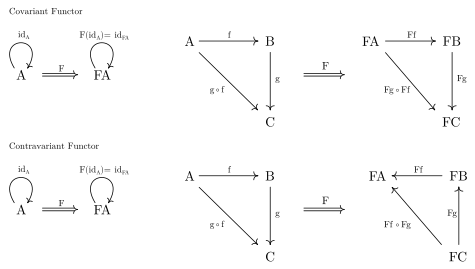
\includegraphics[width=0.6\textwidth]{./figs/Functor.pdf}
			\end{center}
			\caption{Diagrams showcasing the properties of functors.}
			\label{fig:Functor}
		\end{figure}
	\end{definition}

\end{frame}

\begin{frame}[fragile]{Category Theory Brief Introduction}
	\begin{definition}[Natural Transformations]
		Let $\mathcal C$ and $\mathcal D$ be categories, and let $F,G:\mathcal C \to \mathcal D$ be functors.
		A natural transformation $\alpha: F \to G$ is such that the following diagram commutes:
		\begin{figure}[H]
			\begin{center}
				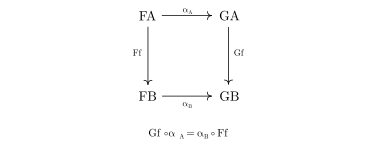
\includegraphics[width=0.60\textwidth]{./figs/NaturalTransformation.pdf}
			\end{center}
			\caption{Commutative diagram of a natural transformation highlighting the commutative property of the definition.}
			\label{fig:NaturalTransformation}
		\end{figure}
	\end{definition}
\end{frame}

\begin{frame}[fragile]{Category Theory Brief Introduction}
	\textbf{Monoids} and \textbf{Monads} are two ubiquitous constructions both in Category Theory and
	Functional Programming. These two concepts will be used when talking about
	data visualization. Therefore, it is required of us to introduce these constructions.

	Let's start with the definition of a monoid in the context of Set Theory.

	\begin{definition}[Monoid - Set Theory]
		A monoid is a triple $(M, \otimes, e_M)$ where $M$ is a set, $\otimes:M\times M \to M$ is a binary operation
		and $e_M$ the neutral element, such that:
		\begin{enumerate}
			\item $a \otimes (b \otimes c) = (a \otimes b) \otimes c$
			\item $a \otimes e_M = e_M \otimes a = a$.
		\end{enumerate}
		\label{def:monoid}
	\end{definition}

	An example of a monoid is $(\mathbb N \cup \{0\}, +, 0)$.
	It is easy to check that the summation operator satisfies the
	associativity neutrality properties.
\end{frame}

\begin{frame}[fragile]{Category Theory Brief Introduction}
	\begin{definition}[Monoid in the  category $\mathbf{Set}$]
		A monoid in $\mathbf{Set}$ is a triple $(M, \mu, \eta)$, where $M \in \text{Ob}_\mathbf{Set}$,
		$\mu:M \times M \to M$ and $\eta: 1 \to M$ are two morphisms in $\mathbf{Set}$ satisfying the
		commutative diagrams below. Note that $1$ is the terminal object in $\mathbf{Set}$, i.e.
		the singleton set (which is unique up to an isomorphism).

		\begin{figure}[H]
			\begin{center}
				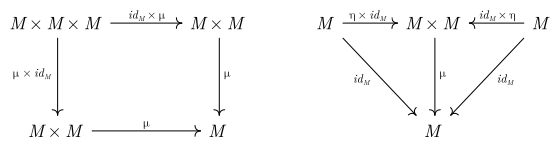
\includegraphics[width=0.7\textwidth]{./figs/MonoidalCategory.pdf}
			\end{center}
			\caption{Commutative diagram for monoid.}
			\label{fig:monoid-diagram}
		\end{figure}
		\label{def:monoid-cat}
	\end{definition}
\end{frame}

\begin{frame}[fragile]{Category Theory Brief Introduction}
	\begin{definition}[Monad]
		A monad is a monoid in $\mathbf{End}_\mathcal C$, which is the triple $(T, \mu, \eta)$,
		where $T:\mathcal C \to \mathcal C$ is a functor,
		$\mu:T \circ T \to T$ and $\eta: 1 \to T$ are natural transformations in $\mathbf{End}_\mathcal C$ satisfying the
		commutative diagrams below. Note that $1$ is the identity functor in $\mathcal{C}$.
		\begin{figure}[H]
			\begin{center}
				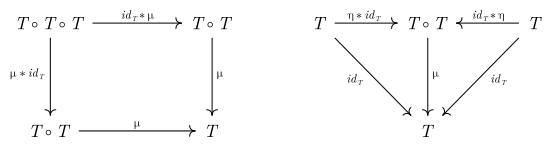
\includegraphics[width=0.7\textwidth]{../notebooks/Monad.pdf}
			\end{center}
			\caption{Commutative diagram for monad.}
			\label{fig:monad}
		\end{figure}
	\end{definition}
\end{frame}

%------------------------------------------------

\begin{frame}{References}
    \footnotesize
    \bibliography{reference.bib}
    \bibliographystyle{apalike}
\end{frame}

%------------------------------------------------

\begin{frame}
    \Huge{\centerline{\textbf{The End}}}
\end{frame}

%----------------------------------------------------------------------------------------

\end{document}
